	\section{Exact Algorithm}
	\label{sec:opt}

	In this section we give an exact algorithm for finding an exact
	bipartitioning of a matrix, extending the branch and bound
	algorithm by Pelt \&
	Bisseling \cite{pelt15}. We first give a quick overview
	of their approach, though
	a better understanding can be gained by reading the
	paper itself.

	After that we give two new bounds that extend the reach of the previous
	algorithm.

	\subsection{Previous work}

	All of this subsection concerns work done in \cite{pelt15}.

	Recall that a branch and bound algorithm initially starts with
	(a representation of) the whole solution space, and then repeatedly
	branches on properties of the solutions until these are refined
	enough that they specify a single solution (this is a leaf in the branch
	and bound tree). When the properties are
	chosen carefully, we may cut off (`bound') large parts of the search
	tree.

	In the case of matrix bipartitioning, a first obvious choice would 
	be to branch on
	which side of the partition we put each nonzero in. For an $n \times m$
	matrix with $N$ nonzeros this results in $2^N$ leaf nodes. However,
	this is not our only option.
	Instead, we can branch of the status of each of the
	rows and columns of the matrix: each of them is either entirely red,
	entirely blue, or `cut', i.e. it contains both colors. As a result, we
	only have $3^{n+m}$ leafs, which is already smaller than $2^N$ when
	$n + m < \log_3(2) N \approx 0.63N$. In fact, not all of the $3^{n+m}$
	states are even reachable: if a row and column intersect in a nonzero,
	we cannot mark one of them as \textit{red} and one of them as \textit{blue}
	(i.e. we do require assignments be consistent).

	When we traverse the branch and bound tree, at each stage we have a
	`partial assignment', where some of the rows and columns are
	\textit{red}, \textit{blue} or \textit{cut}, and some are still
	unassigned. For a given matrix $M$ and its bipartite graph representation
	$G(M) = (V, E)$ (recall the equivalence from \autoref{sec:np}),
	we will write $R \subseteq V$ (resp. $B, C \subseteq V$)
	for the vertices (corresponding to rows and columns) that were assigned
	\textit{red} (resp. \textit{blue}, \textit{cut}). Additionally, while
	all remaining vertices are unassigned, they may still be connected to
	vertices in $R, B$ and $C$. For example, if an unassigned column
	vertex $u$ is
	adjacent to a row vertex in $r \in R$, this means that $M_{ru}$ is nonzero.
	In particular, since row $r$ is red, we cannot make $u$ blue. So we will
	call $u$ \textit{partially red}, with the corresponding subset of $V$
	written as $P_R$ (with $P_B$ defined
	analogously). Finally, an unassigned vertex may have neighbours in both
	$R$ and $B$. While unassigned, we are basically forced to cut this vertex.
	Because of this, we assume that whenever such a vertex is created, we
	immediately cut it. So we will ignore these vertices.

	For pruning, the following two lower bounds on solution cost are used:
	\begin{enumerate}
		\item[] \textbf{Packing bound} Let $E(R)$ denote all the edges that
				are colored red by the current partial assignment (that is, all
				edges adjacent to a vertex in $R$).
				For each partially red vertex
				$p \in P_R$ (i.e. $p$ has a vertex in $R$ adjacent), let
				$$N^R(p) = \{\, e \in E \,\mid\, \text{$e$ is adjacent to $p$
				but not to $R$ or $B$}\,\}$$
				Then all edges in $N^R(p)$ are still free, but directly
				adjacent to a red edge, since $p$ is adjacent to some $r\in R$,
				so we are forced to color $\{p, r\}$ red.

				If we don't want to cut any more vertices, we have to color all
				edges in $N^R(p)$ red. But if
				$|E(R)| + \sum_{p\in P_R} |N^R(p)| > \frac{1}{2}|E|$, this will
				lead to an unbalanced partition, and we are forced to color
				some of the edges in question blue, cutting some
				of the vertices $p \in P_R$ in the process.
				Since we are looking for a lower
				bound, we can greedily take those vertices with largest
				$|N^R(p)|$ until the sum is small enough again.

				Note that we implicitly assumed all the $N^R(p)$ were disjoint,
				so we can assign their edges independently. Since
				$G(M) = (V,E)$ is bipartite, this is true if we consider each
				side of the bipartition separately (that is, the rows and the
				columns). We can then do the same
				for $P_B$, and add everything together to get the
				\textit{packing bound}.
		\item[] \textbf{Matching bound} Let's consider some $p \in P_R$ and
				$q \in P_B$ with $\{p, q\} \in E$. We note that $p$ has a red
				edge adjacent (through its adjacent vertex in $R$), and $q$ has
				a blue edge adjacent. Clearly no matter what color we give
				$\{p, q\}$, we will have to cut one of them.

				We can improve this by finding a maximal set of such edges that
				are disjoint (this is necessary, since otherwise we could
				resolve $\{p, q\}$ and $\{p, q'\}$ just by cutting $p$).
				The relevant graph is just our bipartite graph
				$G(M) = (V, E)$ restricted to
				$P_R \cup P_B \subseteq V$, keeping only edges with one
				endpoint in $P_R$ and one in $P_B$. Bipartite
				matching is a classical problem we can solve in polynomial
				time. Then the size of the maximum matching is a lower bound
				on the number of vertices that still have to be cut by any
				extension of the current partial assignment.
	\end{enumerate}

	These two bounds conflict with each other, so must take the maximum of the
	two. We add to this the total number of already cut vertices $|C|$ to
	obtain a lower bound on any extension of the current partial assignment.
	If this matches the cost of the best solution already seen (an obvious
	upper bound on the optimal solution), we can prune the current subtree.

	One issue with these two bounds is that they are in some sense `local'
	bounds. They both only consider the direct neighbourhoods of $R$ and $B$
	(through $P_R$ and $P_B$). The two bounds we give next can be seen as
	extending the above bounds to the whole graph, taking full advantages of
	its connectivity.

	\subsection{Flow Bound}

	We will begin by extending the matching bound to the whole graph. The
	matching bound considers edges that are adjacent to both red and blue
	edges (through $P_R$ and $P_B$). But there is no need to consider just
	a single edge, and this is especially obvious when we consider the graph
	formulation of the problem.

	Consider a path from $P_R$ to $P_B$ avoiding $R \cup B \cup C$, that is,
	a series of vertices $v_1, v_2, \dots, v_k$ with
	$v_i \not\in R\cup B\cup C$ for $1 \leq i\leq k$,
	and in particular $v_1 \in P_R$ and $v_k \in P_B$,
	such that $\{v_i, v_{i+1}\} \in E$ for all $1 \leq i < k$. This
	corresponds to a series of intersecting rows and columns, the first of
	which contains a red nonzero (corresponding to the edge between $v_1$ and
	its neighbour in $R$) and the last a blue nonzero.

	Clearly then any extension of the current partial assignment must cut one
	of these vertices. If $v_1$ is not cut then it must be fully red, making
	$v_2$ partially red, etc..

	So if a single path between $P_R$ and $P_B$ implies that we have to cut at
	least one vertex, how do we extend this to multiple paths? Here we run in
	to the same issue as with the matching bound: if we have two paths that
	share a vertex, we can just cut that vertex to separate red and blue edges,
	for a cost of $1$.

	\begin{figure}[h]
		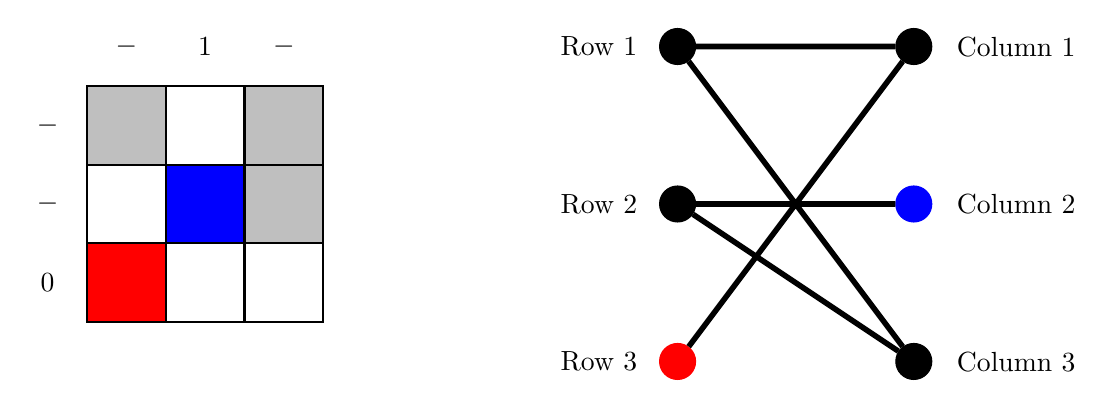
\begin{tikzpicture}[box/.style={rectangle,draw=black,thick, minimum size=1cm}]

\begin{scope}[shift={(-7, 1)}]
\foreach \x in {0,1,2}{
	\foreach \y in {0,1,2}
		\node[box] at (\x,\y){};
}
\node[box,fill=red] at (0,0){};
\node[box,fill=lightgray] at (0,2){};
\node[box,fill=blue] at (1,1){};
\node[box,fill=lightgray] at (2,1){};
\node[box,fill=lightgray] at (2,2){};
\node[] at (-1, 0) {$0$};
\node[] at (-1, 1) {$-$};
\node[] at (-1, 2) {$-$};
\node[] at (0, 3) {$-$};
\node[] at (1, 3) {$1$};
\node[] at (2, 3) {$-$};
\end{scope}

\node[shape=circle,fill=red  ,draw=red  ,minimum size=13pt] (1) at (0, 0) {};
\node[shape=circle,fill=black,draw=black,minimum size=13pt] (4) at (3, 0) {};
\node[shape=circle,fill=black,draw=black,minimum size=13pt] (2) at (0, 2) {};
\node[shape=circle,fill=blue ,draw=blue ,minimum size=13pt] (5) at (3, 2) {};
\node[shape=circle,fill=black,draw=black,minimum size=13pt] (3) at (0, 4) {};
\node[shape=circle,fill=black,draw=black,minimum size=13pt] (6) at (3, 4) {};

\node[] at(-1, 0) {Row $3$};
\node[] at(-1, 2) {Row $2$};
\node[] at(-1, 4) {Row $1$};
\node[] at( 4.3, 0) {Column $3$};
\node[] at( 4.3, 2) {Column $2$};
\node[] at( 4.3, 4) {Column $1$};

\draw[line width=2pt] (1) -- (6) -- (3) -- (4) -- (2) -- (5);

\end{tikzpicture}

		\centering
		\label{fig-flow}
		\caption{Looking at the matrix, it is not a priori clear that row 3
			and column 2 are connected. In the graph representation of the
			matrix we can clearly see the connecting path.}
	\end{figure}

	Hence, to prove a lower bound of more than $1$ we have to require that the
	paths are disjoint. In particular, the
	strongest lower bound we can find will be the maximum number of vertex
	disjoint paths between $P_R$ and $P_B$. Note that these paths must be
	vertex disjoint in $P_R$ and $P_B$ as well, since those vertices may also
	still be cut. Alternatively, when we imagine $R$ and $B$ as a single
	vertex, we are looking for a maximum number of paths from $R$ to $B$ that
	are vertex disjoint outside of $R$ and $B$. In fact, a theorem by Menger
	shows that this is actually exactly the size of the smallest vertex cut.

	\begin{theorem}{(Menger, \cite{menger1927allgemeinen})}
		Let $G$ be a finite undirected graph, and let $u$ and $v$ be two
		non-adjacent vertices in $G$, then the size of the smallest vertex cut
		separating $u$ and $v$ equals the maximum number of vertex disjoint
		paths between $u$ and $v$.
	\end{theorem}

	Unfortunately, the resulting cut may be very unbalanced, so we can only
	use this as an upperbound.

	\subsubsection{Implementation notes on the Flow Bound}

	Finding a maximal set of vertex disjoint paths is a classical maximum flow
	problem, that can be solved by duplicating each vertex and connecting them
	with a capacity $1$ edge, to enforce that every vertex be used only once.
	Specifically, given our graph $G = (V, E)$ we create
	a new directed graph $G' = (V', A)$ with two vertices $v_{in}$, $v_{out}$
	for every $v \in V$, arcs $(u_{out}, v_{in})$ for every $\{u, v\} \in E$,
	and finally we add the arc $(u_{in}, u_{out})$ for every $u \in V$.
	Giving all arcs integer capacities, then the maximum flow between
	$u_{out}$ and $v_{in}$ in $G'$ gives us the minimum vertex cut between
	$u$ and $v$ in $G$.
	A more thorough exposition may be found in \cite{thomas2001introduction}
	in chapter 26.

	However, while the maximum flow problem may be solved in polynomial time,
	it still requires computation over the entire graph, which may slow down
	our algorithm for large matrices. Instead, we can reuse the flow from the
	previous branch and bound step and incrementally recompute the new flow.

	We will state, for the sake of completeness,
	without exposition, how to do this for each change. Suppose
	our branch and bound algorithm selects $u$, and that we already have the
	corresponding maximum flow for our current partial assignment.
	\begin{enumerate}
		\item[] \textbf{Coloring $u$ red} This means the relevant vertex
			becomes a source for the maximum flow problem ($u_{out}$
			specifically). Hence, any new paths will have this vertex as their
			source, and we can just repeatedly do a breadth first search from
			this vertex to find an augmenting path (as opposed to searching
			from all sources, as when we would compute the flow from scratch).
		\item[] \textbf{Uncoloring $u$ red} Now $u_{out}$ is the source of 
			some flow paths. We would like to maintain as many of these as
			possible (to keep our flow maximal). To this end, we temporarily
			pretend that $u_{out}$ is a sink, and find reverse augmenting paths
			to other sources. This we can also do in a single breadth first
			search per unit change in flow. Once this is no longer possible,
			we instead search for sinks to remove flow paths (decrementing the
			flow for each path we find).
		\item[] \textbf{Cutting $u$} This means completely taking $u$ out of
			the flow graph, since the paths for our Flow Bound may not run
			through $C$. However, at most a single path is running through
			$u$, which we could check by looking at the current flow through
			$(u_{in}, u_{out})$. If there is a flow, we can scan from $u_{in}$
			to search for $u_{out}$ (not using the arc that connects them) to
			reroute the flow path in question. If possible, we augment this
			path. If not, we scan for an augmenting path to a source starting
			from $u_{in}$ and a reverse augmenting path to a
			sink starting from $u_{out}$ so we can remove one flow path. We
			then set the capacity of $(u_{in}, u_{out})$ to $0$. This requires
			at most three breadth first searches.
		\item[] \textbf{Uncutting $u$} Any new augmenting path would have to
			run through $u$, and clearly there can be at most one. So we scan
			for a reverse augmenting path to a source from $u_{in}$ and an
			augmenting path to a sink from $u_{out}$. If we find both, we can
			concatenate them and augment this path, incrementing our flow by
			one.
	\end{enumerate}

	The cases for coloring and uncoloring blue vertices are symmetric, so we
	will omit them.
	Note that the reason we can readjust flow paths by single breadth first
	searches is that all arcs have unit capacities.

	\subsection{Extended Packing Bound}

	\todo{Write this whole section}

	We now consider the problem of extending the packing bound over the whole
	graph (rather than just neighbourhoods of $R$ and $B$). This idea is based
	on a similar \todo{cite}

	Instead of looking only at free edges directly incident to vertices in
	$P_R$, we instead look at whole adjacent subgraphs.

	

	\begin{definition}
		Given a graph $(V, E)$ with a partial assignment $R, B, C \subseteq V$,
		then an $R$-adjacent subgraph $(V', E')$ is a tuple of subsets
		$V' \subseteq V$, $E' \subseteq E$, satisfying the following
		properties:
		\begin{itemize}
			\item x
		\end{itemize}
	\end{definition}

	Note that the definition explicitly does not require us to add leaf
	vertices to the subgraph. We can now use these subgraphs to find a lower
	bound on any extension of our partial assignment.

	We do this much the same way 

	\subsubsection{Implementation notes on the Extended Packing Bound}
	\todo{interaction with flow?}

	\subsection{Further implementation notes}

	In this section, in the interest of reproducibility, we make a few notes
	on relevant decisions we made regarding implementation of the branch and
	bound algorithm.

	\subsubsection{Branching strategy}
	While we already specified that we branch on marking a row or column as
	\textit{red}, \textit{blue} or \textit{cut}, the order in which we
	select the rows and columns for branching could significantly affect the
	performance of the algorithm.

	Intuitively, it makes sense to branch on rows and columns with more free
	nonzeros, since their assignment affects the balance of the bipartitioning
	the most, and their high connectivity suggests they may be useful as
	sources of paths in the Flow Bound or subgraphs in the Extended Packing
	Bound. Thus, at each step we select for branching a row or column $u$
	with a maximal
	number of unassigned nonzeros, breaking ties arbitrarily. Additionally,
	since the goal is to cut as few rows and columns as possible, we traverse
	the `\textit{cut}' subtree last, and since the goal is to balance the
	bipartition, we traverse first the subtree that assigns $u$ to the smallest
	side in the bipartition.

	As a footnote we will refer to the paper by Mumcuyan et. al.
	(\cite{mumcuyan18}) who show
	other branching strategies can be faster, and learn to predict the optimal
	strategy based matrix statistics.
	
	\subsubsection{Initial upper bound}

	To correctly prune, our branch and bound algorithm needs an upper bound to
	compare its lower bound against. Before we have found our first feasible
	solution we could use the trivial $\min(n, m) + 1$ lower bound. Although
	this upper bound is in some sense tight (consider an odd square matrix
	with only one nonzero), it is usually quite bad and forces our algorithm
	to consider many very suboptimal solutions before arriving at better ones.

	Instead, we would like to run the algorithm with an upper bound as tight
	as possible. Hence, we run our algorithm with an initial (strict) upper
	bound of $U_1 = 1$, and rerun with
	$U_{i+1} = \lceil \frac{5}{4} U_i \rceil$ until we have found a solution.
